
\section{代数间奏：\trJordan--\trHolder{}套餐}

群论中的\trJordan--\trHolder{}定理，是一个更为基本、而且不知怎么却更为简单的故事的一部分。\trJordan--\trHolder{}「瑜伽」（yoga）\footnote{译注：yoga（瑜伽）是数学家的行话，指一整套融会贯通的心法。}说明了为什么你常常能把某种代数对象分解成素因子或不可约因子，而且分解是唯一的（在恰当的意义下），并且无论你怎么分解，每个素因子／不可约因子出现的次数都相同。从这个观点看，它推广了整数的\trFactorial；\trVectorSpace{}的\trDimension{}的良定性；\trFinitelyGenerated\trAbelianGroups{}的分类；\trDedekind\trIntegralDomain{}中理想的\trFactorial；以及群论中传统的\trJordan--\trHolder{}定理。

我们最感兴趣的将是\trRing{}上的\trModule，但在一般的\trAbelianCategory{} $\scr{C}$ 中工作亦无妨。（这件事还能轻易地进一步推广，见练习~6.5.G。）

我们称对象 $M\in\scr{C}$ 是\textbf{\trSimple}（simple）的（或称\textbf{\trIrreducible}的），若它仅有的\trSubobject{}是 $0$ 与它自身。$M$ 的一条\textbf{\trCompositionSeries{}}（composition series）是一条（有限的）滤过
\begin{equation*}\tag{6.5.0.1}\label{eq:composition-series-filtration}
0=X_0\subsetneq X_1\subsetneq\cdots\subsetneq X_{n-1}\subsetneq X_n=M
\end{equation*}
使得诸商 $X_{i+1}/X_i$ 全是单的。若 $M$ 有一条\trCompositionSeries{}，则称 $M$ 具有\textbf{\trFiniteLength{}}（finite length）。

\textbf{6.5.1. \trJordan--\trHolder{}\trhTheorem。}\ ——\ \emph{若 $M$ 有一条有限\trCompositionSeries{}，则 $M$ 的一切\trCompositionSeries{}都具有相同的\trLength{}，并且诸商全都相同，至多重新排列次序。}

\textbf{6.5.2.}\ \emph{\trhDefinition{}。}\quad 我们把 $M$ 的任何一条\trCompositionSeries{}的\trLength{}称为 $M$ 的\textbf{\trLength{}}（length），记作 $\ell(M)$。由\trJordan--\trHolder{}定理，这一观念是良定的。但我们甚至还有一个更精细的观念：我们还掌握着每个单对象在 $M$ 的任何一条\trCompositionSeries{}中出现的重数。

若 $M$ 不具有\trFiniteLength{}，则我们说 $\ell(M)=\infty$。

\textbf{6.5.3.}\ \emph{\trhExample{}。}\quad 在\trAbelianGroups{}的\trCategory{}中，具有\trFiniteLength{}的对象正是\emph{有限}的\trAbelianGroups。此时把\trJordan--\trHolder{}定理用于 $\mathbb{Z}/n\mathbb{Z}$，便可用它给出 $n$ 的\trFactorial。

\textbf{6.5.4. \trJordan--\trHolder{}定理~6.5.1 的证明。}

设对象 $M\in\scr{C}$ 有两条有限\trCompositionSeries{}：\eqref{eq:composition-series-filtration} 与
\[
0=Y_0\subsetneq Y_1\subsetneq\cdots\subsetneq Y_{p-1}\subsetneq Y_p=M.
\]
作一个矩形阵列，以其诸格中之项为 $Z_{i,j}:=X_i\cap Y_j$，如图~\ref{fig:jordan-holder-array} 所示。图~\ref{fig:jordan-holder-table} 展示了把这一构造施用于 $\mathbb{Z}$-\trModule{} $\mathbb{Z}/(12)$ 的两条\trCompositionSeries{}
\[
(12)\subsetneq(6)\subsetneq(2)\subsetneq(1) \qquad\text{以及}\qquad (12)\subsetneq(4)\subsetneq(2)\subsetneq(1)
\]
的结果。

\begin{figure}[htbp]
\centering
\begin{tikzpicture}[x=1cm,y=1cm,every node/.style={font=\footnotesize}]
  \draw[black!50] (0,0) -- (0,5.35) (1.1,0) -- (1.1,5.35) (2.0,0) -- (2.0,5.35)
    (2.9,0) -- (2.9,5.35) (3.7,0) -- (3.7,5.35) (4.45,0) -- (4.45,5.35)
    (5.2,0) -- (5.2,5.35) (6.2,0) -- (6.2,5.35) (7.1,0) -- (7.1,5.35);
  \draw[black!50] (0,0) -- (7.1,0) (0,0.6) -- (7.1,0.6) (0,1.45) -- (7.1,1.45)
    (0,2.4) -- (7.1,2.4) (0,2.95) -- (7.1,2.95) (0,3.9) -- (7.1,3.9)
    (0,4.75) -- (7.1,4.75) (0,5.35) -- (7.1,5.35);
  \draw[line width=1.5pt]
    (4.45,2.95) -- (4.45,2.4)   (4.45,2.95) -- (7.1,2.95)
    (3.7,2.4) -- (7.1,2.4)      (3.7,2.4) -- (3.7,0)
    (6.2,4.75) -- (7.1,4.75)    (6.2,3.9) -- (7.1,3.9)
    (6.2,1.45) -- (7.1,1.45)    (6.2,0.6) -- (7.1,0.6)
    (1.1,0) -- (1.1,0.6) (2.0,0) -- (2.0,0.6) (2.9,0) -- (2.9,0.6)
    (5.2,0) -- (5.2,0.6) (6.2,0) -- (6.2,0.6);
  \node at (0.55,5.05) {$Z_{0,0}=0$};
  \node at (1.55,5.05) {$0$};
  \node at (2.45,5.05) {$0$};
  \node at (4.075,5.05) {$\cdots$};
  \node at (5.7,5.05) {$0$};
  \node at (6.65,5.05) {$0$};
  \node at (0.55,4.32) {$0$};
  \node at (1.55,4.47) {$Z_{1,1}=$};
  \node at (1.55,4.14) {$X_1\cap Y_1$};
  \node at (2.45,4.47) {$Z_{1,2}=$};
  \node at (2.45,4.14) {$X_1\cap Y_2$};
  \node at (4.075,4.32) {$\cdots$};
  \node at (5.7,4.47) {$X_1\cap$};
  \node at (5.7,4.14) {$Y_{p-1}$};
  \node at (6.65,4.32) {$X_1$};
  \node at (0.55,2.675) {$\vdots$};
  \node at (1.55,2.675) {$\vdots$};
  \node at (2.45,2.675) {$\vdots$};
  \node at (0.55,1.02) {$0$};
  \node at (1.55,1.02) {$X_{n-1}\cap Y_1$};
  \node at (2.45,1.02) {$X_{n-1}\cap Y_2$};
  \node at (5.7,1.18) {$X_{n-1}\cap$};
  \node at (5.7,0.86) {$Y_{p-1}$};
  \node at (6.65,1.02) {$X_{n-1}$};
  \node at (0.55,0.3) {$0$};
  \node at (1.55,0.3) {$Z_{n,1}=Y_1$};
  \node at (2.45,0.3) {$Y_2$};
  \node at (5.7,0.3) {$Y_{p-1}$};
  \node at (6.65,0.3) {$M$};
  \node at (0.55,5.62) {$0=Y_0$};
  \node at (1.55,5.62) {$Y_1$};
  \node at (2.45,5.62) {$Y_2$};
  \node at (4.075,5.62) {$\cdots$};
  \node at (5.7,5.62) {$Y_{p-1}$};
  \node at (6.65,5.62) {$Y_p=M$};
  \node at (-0.62,5.05) {$0=X_0$};
  \node at (-0.55,4.32) {$X_1$};
  \node at (-0.5,2.675) {$\vdots$};
  \node at (-0.68,1.02) {$X_{n-1}$};
  \node at (-0.75,0.3) {$X_n=M$};
  \draw[line width=0.6pt]
    (7.32,2.4) .. controls (7.32,3.05) and (7.36,3.13) .. (7.5,3.15)
    (7.32,3.9) .. controls (7.32,3.25) and (7.36,3.17) .. (7.5,3.15);
  \node at (7.85,3.15) {$\vdots$};
  \draw[line width=0.6pt] \vkbracedown{2.9}{5.2}{-0.15}{0.12}{0.11};
  \node at (4.05,-0.6) {$\cdots$};
\end{tikzpicture}
\caption{\trJordan--\trHolder{}定理证明中的矩形阵列。（依原书手绘图重绘。）}%
\label{fig:jordan-holder-array}
\end{figure}

\begin{figure}[htbp]
\centering
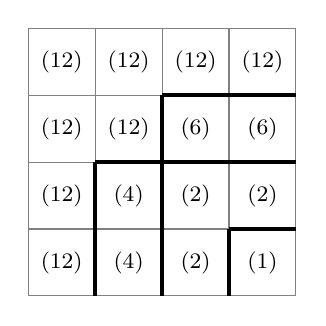
\begin{tikzpicture}[x=1cm,y=1cm,every node/.style={font=\footnotesize}]
  \draw[black!50] (0,0) grid[step=0.85] (3.4,3.4);
  \draw[line width=1.5pt]
    (1.7,2.55) -- (1.7,0)     (1.7,2.55) -- (3.4,2.55)
    (0.85,1.7) -- (3.4,1.7)   (0.85,1.7) -- (0.85,0)
    (2.55,0.85) -- (3.4,0.85) (2.55,0.85) -- (2.55,0);
  \node at (0.425,2.975) {$(12)$};
  \node at (1.275,2.975) {$(12)$};
  \node at (2.125,2.975) {$(12)$};
  \node at (2.975,2.975) {$(12)$};
  \node at (0.425,2.125) {$(12)$};
  \node at (1.275,2.125) {$(12)$};
  \node at (2.125,2.125) {$(6)$};
  \node at (2.975,2.125) {$(6)$};
  \node at (0.425,1.275) {$(12)$};
  \node at (1.275,1.275) {$(4)$};
  \node at (2.125,1.275) {$(2)$};
  \node at (2.975,1.275) {$(2)$};
  \node at (0.425,0.425) {$(12)$};
  \node at (1.275,0.425) {$(4)$};
  \node at (2.125,0.425) {$(2)$};
  \node at (2.975,0.425) {$(1)$};
\end{tikzpicture}
\caption{一张关于 $\mathbb{Z}/(12)$ 两条\trCompositionSeries{}的「\trJordan--\trHolder{}表」样本。（依原书手绘图重绘。）}%
\label{fig:jordan-holder-table}
\end{figure}

\textbf{6.5.5.}\quad 注意到：
\begin{itemize}[leftmargin=2.6em,itemsep=2pt,topsep=3pt]
\item $Z_{i,j}\subset Z_{i',j'}$，若 $i\le i'$ 且 $j\le j'$；
\item $Z_{n,j}=Y_j$，且 $Z_{i,p}=X_i$；
\item $Z_{0,j}=Z_{i,0}=0$；以及
\item $Z_{i,j}\cap Z_{i',j'}=Z_{\min(i,i'),\min(j,j')}$。
\end{itemize}

\textbf{6.5.A.（练习）}\quad （对 $i$ 作\trDescendingInduction{}）证明：$Z_{i,j}/Z_{i,j-1}$ 或者为 $0$，或者同构于单成员 $Y_j/Y_{j-1}$。

类似地，对 $Z_{i,j}/Z_{i-1,j}$ 也有类似的陈述。在这张矩形阵列中，若这两个（横向或纵向相邻的）格中之项的商非零，就在二者之间画一条\emph{粗线}，并用该单群的（\trIsomorphismClass{}）为这条线作标记（仍见图~\ref{fig:jordan-holder-array}）。

考虑该阵列中任何一个 $2\times 2$ 子方块：
\[
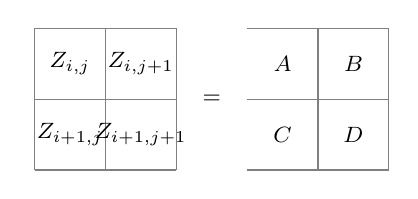
\begin{tikzpicture}[baseline={(current bounding box.center)},every node/.style={font=\footnotesize}]
  \draw[black!50] (0,0) grid[step=0.9] (1.8,1.8);
  \node at (0.45,1.35) {$Z_{i,j}$};
  \node at (1.35,1.35) {$Z_{i,j+1}$};
  \node at (0.45,0.45) {$Z_{i+1,j}$};
  \node at (1.35,0.45) {$Z_{i+1,j+1}$};
  \node at (2.25,0.9) {$=$};
  \draw[black!50] (2.7,0) grid[step=0.9] (4.5,1.8);
  \node at (3.15,1.35) {$A$};
  \node at (4.05,1.35) {$B$};
  \node at (3.15,0.45) {$C$};
  \node at (4.05,0.45) {$D$};
\end{tikzpicture}
\]
我们将看到，方块内部的诸粗线必构成如下五种花样之一（每一种都在图~\ref{fig:jordan-holder-table} 中出现过）。
\[
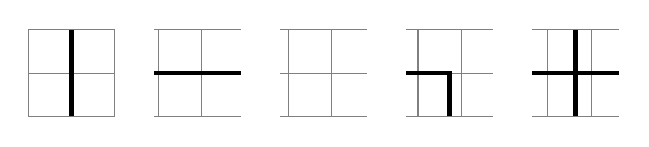
\begin{tikzpicture}[baseline={(current bounding box.center)},every node/.style={font=\footnotesize}]
  \draw[black!50] (0,0) grid[step=0.55] (1.1,1.1);
  \draw[line width=1.5pt] (0.55,0) -- (0.55,1.1);
  \draw[black!50] (1.6,0) grid[step=0.55] (2.7,1.1);
  \draw[line width=1.5pt] (1.6,0.55) -- (2.7,0.55);
  \draw[black!50] (3.2,0) grid[step=0.55] (4.3,1.1);
  \draw[black!50] (4.8,0) grid[step=0.55] (5.9,1.1);
  \draw[line width=1.5pt] (4.8,0.55) -- (5.35,0.55) -- (5.35,0);
  \draw[black!50] (6.4,0) grid[step=0.55] (7.5,1.1);
  \draw[line width=1.5pt] (6.95,0) -- (6.95,1.1) (6.4,0.55) -- (7.5,0.55);
\end{tikzpicture}
\]
由 $A=B\cap C$ 可见：(i) 若 $D=B$，则 $A=C$；(ii) 若 $D=C$，则 $A=B$。这便处置了前三种情形。

再设 $D/B$ 与 $D/C$ \emph{都}非零（从而是单的）。若 $B=C$，我们便处于第四种（「肘形」）情形。

最后，若不然，我们将看到 $D/B\cong C/A$（类似地，$D/C\cong B/A$），于是我们便处于第五种情形。考虑映射 $C\to D/B$。那么由 $A=B\cap C$（\S6.5.5），$A$ 恰是这个映射的\trKernel。于是我们有一个\trMonomorphism{} $C/A\hookrightarrow D/B$。由 $D/B$ 的单性，要么 $C/A$ 为零，要么这个\trMonomorphism{}实际上是一个\trIsomorphism{} $C/A\overset{\sim}{\hookrightarrow}D/B$。\hfill$\square$

\textbf{6.5.B.（练习）}\quad 证明\trJordan--\trHolder{}定理。提示：注意到那些加粗的线可以解释为一些路径：从表的右缘出发、走到表的底部、途中恰拐一次左弯。这将给出一个\trBijection，把一条滤过的诸单商对应到另一条滤过的诸单商。

\textbf{6.5.C.（练习）}\quad 证明：\trFiniteLength{}对象 $M$ 的每个\trSubquotient{}都具有\trFiniteLength{}。一条可能的进路：设该\trSubquotient{}为 $M''/M'$，其中 $M'\subseteq M''\subseteq M$。为 $M$ 选定一条\trCompositionSeries{} $M_\bullet$。用类似的方式再作一张新的矩形表，这次使用\trCompositionSeries{} $M_\bullet$ 与滤过 $0\subseteq M'\subseteq M''\subseteq M$。仿照\trJordan--\trHolder{}定理之证明的进路，对路径作合适的思考。

\textbf{6.5.D.（练习）}\quad 证明：\trLength{}在\trExactSequence{}中是可加的：若 $0\to M'\to M\to M''\to 0$ 是一个\trExactSequence，则 $\ell(M)=\ell(M')+\ell(M'')$。（\emph{不要}假设这些对象都具有\trFiniteLength{}。）

\textbf{6.5.E.（练习）}\quad 证明：\trFiniteLength{}\trModule{}的任何一条滤过都能\trRefine{}成一条\trCompositionSeries{}。

\textbf{6.5.F.（不重要的练习）}\quad 证明：$\scr{C}$ 中具有\trFiniteLength{}的诸对象构成 $\scr{C}$ 的一个\trFullSubcategory。

由\trGroup{}组成的\trCategory{}并不构成一个\trAbelianCategory，故定理~6.5.1 不能直接推出群的传统\trJordan--\trHolder{}定理。不过，同一个证明无须改动即可适用，只是要多加一个输入。

\textbf{6.5.G.（我们不会用到的练习）}\quad 证明群的\trJordan--\trHolder{}定理。你将需要\trSecondIsomorphismTheorem{}（second isomorphism theorem）：若 $N_1$ 与 $N_2$ 是\trGroup{} $G$ 的两个\trNormalSubgroup{}（normal subgroups），则 $N_1N_2$ 构成 $G$ 的一个\emph{正规}子群，且 $N_2/(N_1\cap N_2)\cong(N_1N_2)/N_1$。

\textbf{6.5.6. 若干只对环上的模才特有的补充事实。}

现在我们把这些概念专门用于\trCategory{} $\catMod{A}$。

\textbf{6.5.H.（练习）}\quad 证明：$\catMod{A}$ 的单对象恰是形如 $A/\mathfrak{m}$ 的那些对象，其中 $\mathfrak{m}$ 是 $A$ 的一个\trMaximalIdeal。

\textbf{6.5.I.（练习）}\quad 设 $M$ 是一个\trFiniteLength{}的 $A$-\trModule，而 \eqref{eq:composition-series-filtration} 是 $M$ 的一条\trCompositionSeries{}，其中 $M_i/M_{i-1}\cong A/\mathfrak{m}_i$（诸 $\mathfrak{m}_i$ 是\trMaximalIdeal，未必互不相同）。证明：$M$ 被 $\mathfrak{m}_1\cdots\mathfrak{m}_n$ \trAnnihilate{}。等价地，$M$ 是一个 $A/(\mathfrak{m}_1\cdots\mathfrak{m}_n)$-\trModule。

现在设列表 $(\mathfrak{m}_1,\dots,\mathfrak{m}_n)$ 由互不相同的\trMaximalIdeal{} $\mathfrak{n}_1,\dots,\mathfrak{n}_s$ 组成，它们分别以重数 $\ell_1,\dots,\ell_s$ 出现。（这些正是定义~6.5.2 中提到的「精化」\trLength{}。）

由\trChineseRemainderTheorem，
\[
A/\mathfrak{m}_1\cdots\mathfrak{m}_n\cong A/\mathfrak{n}_1^{\ell_1}\cdots\mathfrak{n}_s^{\ell_s}\cong A/\mathfrak{n}_1^{\ell_1}\times\cdots\times A/\mathfrak{n}_s^{\ell_s}.
\]
设 $1\le i\le s$，取 $A$ 中的一个元素 $e_i$，使得 $e_i\equiv 1\pmod{\mathfrak{n}_i^{\ell_i}}$，且当 $i\neq j$ 时 $e_i\equiv 0\pmod{\mathfrak{n}_j^{\ell_j}}$。诸 $e_i$ 的存在性由\trChineseRemainderTheorem{}保证。

\textbf{6.5.J.（练习）}\quad 证明：$M\cong e_1M\times\cdots\times e_sM$，且 $e_iM$ 是一个\trFiniteLength{}的\trModule，其全部单商都是 $A/\mathfrak{n}_i$。于是 $M$ 是若干块的乘积，其中每一块都带有\trCompositionSeries{}，且\trCompositionSeries{}里只有一种类型的「单因子」。

\textbf{6.5.K.（练习）}\quad 设 $M$ 是一个\trFiniteLength{}的 $A$-\trModule。证明：$M$ 是\trFinitelyGenerated{}的，且 $\Supp M$ 由 $\Spec A$ 的有限多个点组成，并且全是\trClosedPoint。（其逆命题将在\trNoetherian{}假设下作为练习~6.6.X(a) 得到证明。）这样，我们便有了「$M$ 在这些闭点中每一点处的\trLength{}」这一观念。

\textbf{6.5.7.}\ \emph{\trhDefinition{}。}\quad 若 $A$ 作为其自身上的\trModule{}具有\trFiniteLength{}，则称 $A$ 是一个\textbf{\trArtinian{}环}（Artinian ring）。若 $A$ 进而还是一个\trLocalRing，则称 $A$ 是一个\textbf{\trArtin{}或\trArtinian{}局部环}（Artin or Artinian local ring）。

\textbf{6.5.8.}\ \emph{把这套语言用于\trScheme{}。}\quad 接下来我们考虑概形 $X$ 上的\trQCSheaf{}之\trCategory{} $\catQCo_X$。对于 $X$ 上\trFiniteLength{}的\trQCSheaf，我们有\trLength{} $\ell(\scr{F})$ 这一观念。

\textbf{6.5.L.（练习）}\quad 证明：$\catQCo_X$ 的单对象恰是那些同构于\trClosedPoint{}的\trStructureSheaf{}的对象。

\textbf{6.5.M.（练习）}\quad 设 $\scr{F}$ 是 $\catQCo_X$ 中一个具有\trFiniteLength{}的成员。证明：$\scr{F}$ 是有限型的，且 $\Supp\scr{F}$ 由 $X$ 的有限多个点组成，并且全是\trClosedPoint。（其逆命题将在\trNoetherian{}假设下作为练习~6.6.X(b) 得到证明。）请说明如何定义 $\scr{F}$ 在 $\Supp\scr{F}$ 中某一点处的\trLength{}。

\textbf{6.5.9.}\ \emph{\trhDefinition{}。}\quad 所谓\textbf{\trScheme{}的\trLength{}}（length of a scheme），就是其\trStructureSheaf{} $\OO_X$（在 $\catQCo_X$ 中）的\trLength{}。若 $\OO_X$ 具有\trFiniteLength{}，则称概形 $X$ 是\textbf{\trFiniteLength{}}的，或称其为\textbf{\trArtinian}的。
